% ============================================================
% PT100 Industrial Thermometer — Project Progress Log
% Team: Pranay, Nehan, and Akshit
%
% This file is a standalone LaTeX document. Keep the image files
% in the same directory as this file, or edit the image paths below.
% ============================================================

\documentclass[12pt,a4paper]{article}

\usepackage[margin=25mm]{geometry}
\usepackage{graphicx}
\usepackage{float}
\usepackage{booktabs}
\usepackage{array}
\usepackage{amsmath}
\usepackage{siunitx}
\usepackage{hyperref}
\usepackage{xcolor}
\usepackage{caption}
\usepackage{enumitem}
\usepackage{tcolorbox}

\usepackage{microtype}
\usepackage{setspace}

\hypersetup{
    colorlinks=true,
    linkcolor=black,
    urlcolor=black,
    citecolor=black
}

\setstretch{1.08}
\setlength{\parskip}{0.55em}
\setlength{\parindent}{0pt}
\renewcommand{\arraystretch}{1.2}

% Include an image if it is present; otherwise show a clear placeholder.
\newcommand{\ProjectImage}[3][0.88\linewidth]{%
    \begin{figure}[H]
        \centering
        \IfFileExists{#2}
            {\includegraphics[width=#1,keepaspectratio]{#2}}
            {\fbox{\parbox[c][35mm][c]{0.82\linewidth}{\centering
             Image file not found: \texttt{\detokenize{#2}}}}}
        \caption{#3}
    \end{figure}
}

\begin{document}

% -------------------- Page 1: Title page --------------------
\begin{titlepage}
    \centering
    \vspace*{1.4cm}
    {\Huge\bfseries Progress Log\par}
    \vspace{1.8cm}
    {\Large\bfseries Made by:\par}
    \vspace{0.6cm}
    {\large Nehan Mohammad\par}
    \vspace{0.25cm}
    {\large T. Pranay Siddarth Reddy\par}
    \vspace{0.25cm}
    {\large Akshit\par}
    \vspace{1.3cm}
    {\Large\bfseries Assigned by:\par}
    \vspace{0.6cm}
    {\large Prof.\ Dr.\ GVV Sharma\par}
    \vfill
    {\large Development of a PT100-Based Digital Thermometer\par}
\end{titlepage}

% -------------------- Page 2: Contents --------------------
\pagenumbering{roman}
\tableofcontents
\clearpage

% -------------------- Page 3: Acknowledgment + Abstract --------------------
\section*{Acknowledgment}
\addcontentsline{toc}{section}{Acknowledgment}
We would like to express our sincere gratitude to our instructor,
Prof.\ Dr.\ GVV Sharma, for assigning this project and guiding us
through its practical implementation. We are also immensely thankful
to our Teaching Assistants---Subhodeep, Vivek, and Jnanesh---for their
continuous support, valuable feedback, and technical assistance during
the lab sessions. Their insights were instrumental in helping us
troubleshoot circuit issues and successfully complete this project.

\vspace{0.8cm}
\noindent\rule{\linewidth}{0.4pt}
\vspace{0.4cm}

\section*{Abstract}
\addcontentsline{toc}{section}{Abstract}
This log records the practical development of our PT100-based digital
thermometer, from understanding the components and testing a standard
character LCD to debugging the complete sensor circuit, transferring it
to perfboard, and designing an enclosure in OpenSCAD. The emphasis is on
the work actually carried out, including the faults encountered and the
checks used to isolate them. The reference paper supplied for the project
also discusses automated data collection and machine-learning calibration;
our implementation instead relied on manual calibration and a direct
resistance-to-temperature calculation on an Arduino.

\clearpage
\pagenumbering{arabic}

\section{Project Objective and Working Principle}

Our objective was to build a compact digital thermometer using a PT100
platinum resistance temperature detector (RTD), an Arduino, and a
16-by-2 character LCD. The PT100 was selected because its resistance
changes predictably with temperature and it is widely used in precision
temperature measurement. Its nominal resistance is \SI{100}{\ohm} at
\SI{0}{\degreeCelsius}. Around ordinary operating temperatures, the
resistance changes by approximately \SI{0.385}{\ohm} per degree Celsius,
so reliable measurement requires attention to the sensing circuit,
connections, and calibration.

The basic measurement chain is:

\begin{enumerate}[leftmargin=2em]
    \item The PT100 resistance changes as its temperature changes.
    \item A resistor-based measurement circuit converts that resistance
    into a voltage that the Arduino's analogue input can read.
    \item The Arduino averages repeated analogue-to-digital converter
    (ADC) readings and estimates the sensor resistance.
    \item A temperature equation converts the estimated resistance into
    temperature.
    \item The LCD displays the calculated temperature and the compensated
    resistance, while the serial monitor provides additional diagnostic
    values.
\end{enumerate}

The supplied reference material describes more elaborate alternatives,
including a Wheatstone bridge, an external ADS1115 ADC, automated
optical character recognition (OCR), and machine-learning regression.
Those methods were useful background, but they were not the calibration
workflow we followed for this build. Our practical focus was to make the
physical circuit reliable and to calibrate it manually.

\section{Components and Circuit Understanding}

We began by identifying the components and understanding the role of each
part before making permanent connections. The main components were the
Arduino board, PT100 sensor, reference resistor, 16-by-2 parallel LCD,
contrast potentiometer, breadboard, jumper wires, and later a perfboard
for the permanent circuit. The potentiometer adjusts the LCD contrast;
it does not perform the temperature calibration.

\ProjectImage{figs/components.jpeg}
{Components collected for the PT100 thermometer.}

We studied the circuit schematic provided with the reference material to
understand the sensor measurement path and the display connections. The
sensor circuit and the LCD circuit have different jobs: the sensor path
provides a measurable voltage related to resistance, while the LCD path
presents the result to the user. A common ground and correct supply
connections are essential for both sections to work consistently.

\ProjectImage{figs/schematic.jpeg}
{Reference schematic used to understand the measurement and display circuits.}

A key concept was that the Arduino does not measure resistance directly.
It measures voltage at an analogue input. Resistance is inferred from the
voltage-divider relationship and the known reference resistance (with a reference resistance of approximately \SI{120}{\ohm}). Any
unexpected series resistance from leads, jumper wires, or contacts can
therefore affect the result. This became especially relevant during
debugging and calibration.

\section{Testing the LCD}

Before connecting the PT100 measurement circuit, we tested the LCD as a
separate subsystem. We wired the standard parallel LCD directly to the
Arduino, without an I\textsuperscript{2}C backpack, and used a simple
test program to check whether the display could operate independently.

Our tests included:
\begin{itemize}[leftmargin=2em]
    \item printing \texttt{Hello World};
    \item checking whether text could scroll as expected; and
    \item changing the displayed text over time.
\end{itemize}

These tests were intended to separate LCD and wiring problems from any
problems that might later arise in the PT100 measurement code.

\subsection{Jumper wire connection issue}

The LCD did not behave as expected during the first tests. We initially
suspected that the Arduino or the LCD itself might be defective. After
spending considerable time checking the hardware, we traced the problem
to faulty jumper wires. This was an important debugging lesson: a
connection that looks physically correct is not necessarily electrically
continuous.

We learned to verify suspect wires individually and to change only one
part of the setup at a time. Testing the LCD separately was still useful,
because it established a simple baseline before we introduced the sensor
and its measurement code.

\section{Calibration Using Least Squares}
\subsection{Introduction to Calibration}
\textbf{Calibration} is the process of establishing a mathematical relationship between the output of a measuring instrument and a corresponding reference quantity of known value. In sensor applications, calibration enables measured electrical quantities, such as voltage, to be converted into meaningful physical quantities, such as temperature.

When a sensor exhibits a nonlinear voltage--temperature relationship, a polynomial model may be used to approximate its behaviour over a specified operating range. A second-degree polynomial model is given by
\[\boxed{T = Av^2 + Bv + C}\]
where \(T\) is the reference temperature in \(^\circ\mathrm{C}\), \(v\) is the measured sensor voltage in Volts (V), and \(A\), \(B\), and \(C\) are calibration coefficients determined experimentally. Note that our system utilizes a reference resistance of approximately \SI{120}{\ohm}.

\subsection{Experimental Data Collection}
Calibration begins with the collection of experimental data where each observation pairs a sensor voltage with a reference temperature, Note that, the measured data contains 6 decimal points but the least count of ADC is not : \((v_1, T_1), \ldots, (v_N, T_N)\). 

Below is a dataset for our initial calibration dataset containing roughly 7 ADC voltage and temperature measurements (note that this initial dataset led to an average error of 5--6 degrees due to calibration offsets):

\begin{table}[H]
\centering
\begin{tabular}{ccc}
\toprule
Observation \(i\) & temperature \(v_i\) (V) & Voltage \(T_i\) (\(^\circ\mathrm{C}\)) \\
\midrule
1 & 86.3 & 2.520586 \\
2 & 71.6 & 2.474252 \\
3 & 62.5 & 2.437185 \\
4 & 53.6 & 2.404751 \\
5 & 45.5 & 2.376950 \\
6 & 34.8 & 2.331195 \\
7 & 22.4 & 2.284281 \\
\bottomrule
\end{tabular}
\caption{Initial Calibration Dataset   (\(~7\) points, leading to 5--6\(^\circ\mathrm{C}\) error).}
\end{table}

\subsection{Method I: Algebraic Method (Intuition and Formulation)}
For beginners, the algebraic method serves as the most intuitive starting point because it translates physical measurements directly into traditional algebra. 

Imagine plotting your measured voltages on the horizontal axis and reference temperatures on the vertical axis. We want to find a parabola (quadratic curve) that best follows these points. Substituting a specific voltage \(v_i\) and its paired temperature \(T_i\) into our model gives one algebraic equation:
\[Av_i^2 + Bv_i + C = T_i\]

If we have \(N\) experimental observations, we can write down \(N\) such equations. If we only had three data points, we could solve them simultaneously to find a unique parabola passing exactly through all three points. However, real-world sensor measurements always contain small noise and experimental errors. If a single data point is corrupted by noise, forcing the curve to pass through it creates wild inaccuracies elsewhere. 

To utilize all available data and smooth out measurement noise, we collect an overdetermined set of equations (\(N > 3\)). Since no single parabola can pass through every noisy point simultaneously, we define a residual error \(e_i = T_i - (Av_i^2 + Bv_i + C)\) for each point. The least-squares technique minimizes the cumulative squared error across all observations:
\[J(A,B,C) = \sum_{i=1}^{N} \left[T_i - (Av_i^2 + Bv_i + C)\right]^2\]
By finding the coefficients \(A\), \(B\), and \(C\) that minimize \(J(A,B,C)\), we obtain a statistically robust calibration curve that balances all measurements.

\subsection{Method II: Matrix Method (Compact Mathematical Representation)}
While writing out individual algebraic equations is great for conceptual understanding, it becomes extremely tedious when handling dozens of data points. The matrix method streamlines this by packaging the entire system into a compact linear algebra formulation.

For each observation \(i\), we can express the scalar equation as a matrix product:
\[\begin{bmatrix} v_i^2 & v_i & 1 \end{bmatrix} \begin{bmatrix} A \\ B \\ C \end{bmatrix} = T_i\]

When we stack all \(N\) observations together, the individual row vectors combine to form a large design matrix \(X\), the coefficients form a column vector \(\boldsymbol{\theta}\), and the reference temperatures form a vector \(\mathbf{T}\):
\[X = \begin{bmatrix} v_1^2 & v_1 & 1 \\ v_2^2 & v_2 & 1 \\ \vdots & \vdots & \vdots \\ v_N^2 & v_N & 1 \end{bmatrix}, \quad \boldsymbol{\theta} = \begin{bmatrix} A \\ B \\ C \end{bmatrix}, \quad \mathbf{T} = \begin{bmatrix} T_1 \\ T_2 \\ \vdots \\ T_N \end{bmatrix}\]

Thus, the entire calibration problem simplifies to the matrix equation:
\[X\boldsymbol{\theta} \approx \mathbf{T}\]

To solve this least-squares problem geometrically and algebraically, we project the target vector \(\mathbf{T}\) onto the column space of \(X\). This leads directly to the standard normal equations:
\[X^\mathsf{T}X\boldsymbol{\theta} = X^\mathsf{T}\mathbf{T}\]
Assuming the columns of \(X\) are linearly independent, we can invert \(X^\mathsf{T}X\) to solve uniquely for the coefficient vector:
\[\boldsymbol{\theta} = (X^\mathsf{T}X)^{-1}X^\mathsf{T}\mathbf{T}\]
This matrix formulation provides a universal framework that scales effortlessly whether you have 10 data points or 10,000, and it extends directly to higher-order polynomials by simply adding more columns to the design matrix \(X\).

\subsection{Method III: Computational Method Using Python}
In practice, manual matrix inversion can lead to numerical instability and rounding errors. Modern engineering implementations rely on numerical computing libraries like Python's NumPy to solve least-squares problems robustly via advanced matrix decompositions (`np.linalg.lstsq`).

The computational workflow is structured into three logical blocks:
\begin{enumerate}
    \item \textbf{Data Initialization Block:} Sets up the measured sensor voltages and reference temperatures as NumPy arrays.
    \item \textbf{Design Matrix Construction Block:} Uses `texttt{np.column\_stack}` to assemble the squared voltage, linear voltage, and constant columns into the design matrix \(X\).
    \item \textbf{Least-Squares Regression Block:} Invokes NumPy's least-squares solver to extract optimal coefficients \(A\), \(B\), and \(C\).
\end{enumerate}

\begin{tcolorbox}[colback=gray!5!white,colframe=gray!75!black,title=Python: Experimental Data and Design Matrix]
\small
\begin{verbatim}
import numpy as np

# 1. Initialize experimental data arrays
# Voltage measurements in volts (~120 ohm ref setup)
v = np.array([0.50, 0.70, 0.90, 
              1.10, 1.30, 1.50, 1.70])

# Corresponding reference temperatures in degrees Celsius
T = np.array([20.2, 25.1, 29.8, 
              35.3, 41.0, 47.2, 53.1])

# 2. Construct design matrix X containing [v^2, v, 1]
X = np.column_stack((v**2, v, 
                     np.ones_like(v)))
\end{verbatim}
\end{tcolorbox}

The next block computes the regression coefficients by solving the overdetermined system:

\begin{tcolorbox}[colback=gray!5!white,colframe=gray!75!black,title=Python: Coefficient Computation via Least Squares]
\small
\begin{verbatim}
# 3. Solve X * theta = T using least-squares
coefficients, residual_sum, rank, \
    singular_values = np.linalg.lstsq(
        X, T, rcond=None
    )

A, B, C = coefficients
print("A =", A)
print("B =", B)
print("C =", C)
\end{verbatim}
\end{tcolorbox}

Finally, the third block evaluates model accuracy by computing predictions, residuals, and Root Mean Square Error (RMSE), and demonstrates real-time temperature inference:

\begin{tcolorbox}[colback=gray!5!white,colframe=gray!75!black,title=Python: Model Evaluation and Inference]
\small
\begin{verbatim}
# 4. Evaluate fit quality and compute RMSE
T_predicted = A * v**2 + B * v + C
residuals = T - T_predicted
rmse = np.sqrt(np.mean(residuals**2))
print("RMSE =", rmse, "deg C")

# 5. Perform inference for a new voltage reading
v_new = 1.40
T_estimated = A * v_new**2 + \
              B * v_new + C
print("Estimated Temp:", T_estimated)
\end{verbatim}
\end{tcolorbox}
\section{Checking the Completed Breadboard Circuit}

After the circuit was operating, we rechecked the individual connections
with a multimeter. This was not just a final formality: it helped us
confirm electrical continuity and look for unexpected shorts or open
connections before making the arrangement permanent.

We checked the connections methodically, including supply and ground,
LCD signal wiring, the potentiometer connections, and the PT100
measurement path. We also treated the measured resistance as a useful
diagnostic value. A resistance reading that was inconsistent with the
expected sensor path could indicate a poor connection, a wrong connection,
or a short circuit.

\subsection{Troubleshooting corrupted LCD characters}
After integrating the LCD, potentiometer, PT100, and Arduino, the display
showed corrupted characters rather than the intended output. We checked
the circuit again and found two contributing issues: some jumper wires
were damaged, and the LCD data connections had been made in reverse
order. Since the LCD uses several parallel data lines, incorrect ordering
can produce unreadable characters even when the display is powered.

We corrected the wiring and checked the data-pin order against the
connection reference. This reinforced the need to verify every signal
line individually rather than relying only on the apparent neatness of
the circuit.

\ProjectImage{figs/finalbread_circuit.jpeg}
{Integrated PT100 thermometer circuit on the breadboard after the wiring was reorganised.}

\textbf{Intentional pin-layout modification:} we deliberately changed
the LCD pin assignments from those shown in the reference PDF to create
a neater and more practical physical layout. The Arduino sketch was
updated to match the revised wiring. After making the changes, we checked
the connections and tested the LCD signals to confirm that the pins were
working as intended. We also verified the completed program's behaviour
and confirmed that no callback-related errors remained at the end of
testing.


This stage gave us more confidence that the circuit was not merely
displaying plausible numbers by chance. It also provided a useful
baseline for the transfer from breadboard to perfboard, where every
connection would become harder to change.

\section{Moving the Circuit to Perfboard}

After verifying the breadboard circuit, we transferred the design to a
perfboard. The goal was to move from temporary plug-in connections to a
more compact and mechanically stable arrangement suitable for the
thermometer enclosure.

We planned the component positions before completing the soldering. The
layout needed to minimise occupied space while leaving enough room to
route the connections clearly and avoid unintended contact between
conductive points. Compactness was important, but it could not come at
the cost of making the circuit difficult to inspect or repair.

We soldered the header pins such that, it fit perfectly on the arduino, creating a very compact design without use the wires. You can just pop-in the header pins directly to the arduino digital pins quite easily and without the mess of wires getting in the way.

\ProjectImage{figs/finalsolder_circuit.jpeg}
{Soldered circuit arranged on perfboard.}

\subsection{PT100 terminals shorted during soldering}

During soldering, the PT100 terminals were accidentally shorted. The
multimeter then indicated a resistance of approximately
\SI{0}{\ohm}, which was inconsistent with the nominal
\SI{100}{\ohm} PT100 resistance at \SI{0}{\degreeCelsius}. This made
debugging confusing until we considered that the problem might be in the
newly soldered connections rather than in the sensor or the software.

The incident demonstrated why continuity and resistance checks are
necessary after soldering. A solder bridge can bypass the sensing
element and make the circuit appear to have almost no resistance. The
appropriate response is to disconnect power, inspect the solder joints,
remove any unintended bridge, and measure the isolated sensor path again
before reconnecting the circuit.

We used this experience to reinforce our practice of checking the
physical circuit after each significant change instead of assuming that
a circuit which worked on a breadboard will remain correct after
soldering.

\section{Enclosure Design in OpenSCAD}

Once the circuit had been transferred to perfboard, we designed and
modelled an enclosure in OpenSCAD. The aim was to give the electronics
a defined physical form, protect the assembled circuit during ordinary
handling, and make the LCD readable from the front.

The model allowed us to consider the relationship between the board,
display, wiring space, and external dimensions before fabricating a
case. We treated the enclosure as part of the engineering process rather
than as decoration: a useful case must accommodate the real component
dimensions and allow access to the display without placing pressure on
the solder joints or wires.

\ProjectImage{figs/3dmodel_view1.jpeg}
{First view of the thermometer enclosure model in OpenSCAD.}

\ProjectImage{figs/3dmodel-view2.png}
{Additional view of the enclosure model, used to inspect its overall form and layout.}

The modelling stage also made us think about maintainability. A compact
case is valuable only if the circuit can still be assembled, inspected,
and serviced. The final dimensions should therefore be checked against
the actual perfboard, LCD, and cable positions before fabrication.

\section{Calibration, Verification, and Practical Limitations}

Calibration was performed manually rather than through the automated
OCR and machine-learning pipeline described in the reference paper.
The generic PT100 least-squares coefficient method initially led to a noticeable temperature error of 5--6 degrees Celsius. Upon investigation, we discovered that the reference voltage was initially assumed to be 4.7\,V, whereas the actual supply voltage measured directly was 5\,V—an error attributed to a faulty multimeter during preliminary checks.

To rectify this and achieve high precision, we performed a refined final calibration using an expanded dataset of 19 voltage measurements with minimal error. Below is the placeholder for our final calibration dataset table:

\begin{table}[H]
\centering
\begin{tabular}{ccc}
\toprule
Observation \(i\) & Temperature \(v_i\) (V) & Voltage \(T_i\) (\(^\circ\mathrm{C}\)) \\
\midrule
1 & 7.3  & 2.359883 \\
2 & 10.8 & 2.374663 \\
3 & 15.1 & 2.394369 \\
4 & 20.1 & 2.414076 \\ 
5 & 25.8 & 2.438710 \\ 
6 & 30.2 & 2.458416 \\ 
7 & 34.8 & 2.478123 \\
8 & 39.5 & 2.497633 \\
9 & 44.4 & 2.517537 \\
10 & 50.5 & 2.542170 \\
11 & 56.9 & 2.566803 \\
12 & 60.4 & 2.581583 \\
13 & 65.5 & 2.601290 \\
14 & 71.1 & 2.620997 \\
15 & 73.9 & 2.630850 \\ 
16 & 79.4 & 2.650557 \\
17 & 83.2 & 2.665337 \\ 
18 & 90.3 & 2.689971 \\ 
19 & 96.8 & 2.714604 \\




\bottomrule
\end{tabular}
\caption{Final Calibration Table   (\(~19\) voltages with minimal error).}
\end{table}

The reference material explains why calibration matters: the PT100's
resistance-temperature relation is predictable but not perfectly linear,
and small resistance errors can produce noticeable temperature errors.

In our implementation, calibration involved checking the displayed
temperature against a reference thermometer at known or observed
temperatures and adjusting the relevant software parameters as required.
The code contains a reference-resistance value and a lead/contact
correction, so those values must correspond to the assembled hardware.
A calibration result is meaningful only when the sensor and reference
thermometer have had time to approach the same temperature and the
measurements are taken consistently.

The uploaded sketch averages 19 ADC readings to reduce short-term
measurement jitter. Averaging can make a reading steadier, but it does
not by itself remove systematic errors caused by a wrong resistance
value, poor connections, supply variation, sensor placement, or
insufficient calibration. Likewise, a stable LCD reading is not proof
of industrial-grade accuracy. Accuracy must be established by repeated
comparison with a suitable reference over the intended operating range.
\subsection{Project Demonstration}

After tedious verification and calibration, our project was finally completed. Given below are four demonstrations of our thermometer alongside, laboratory grade thermometer.

\begin{figure}[H]
    \centering
    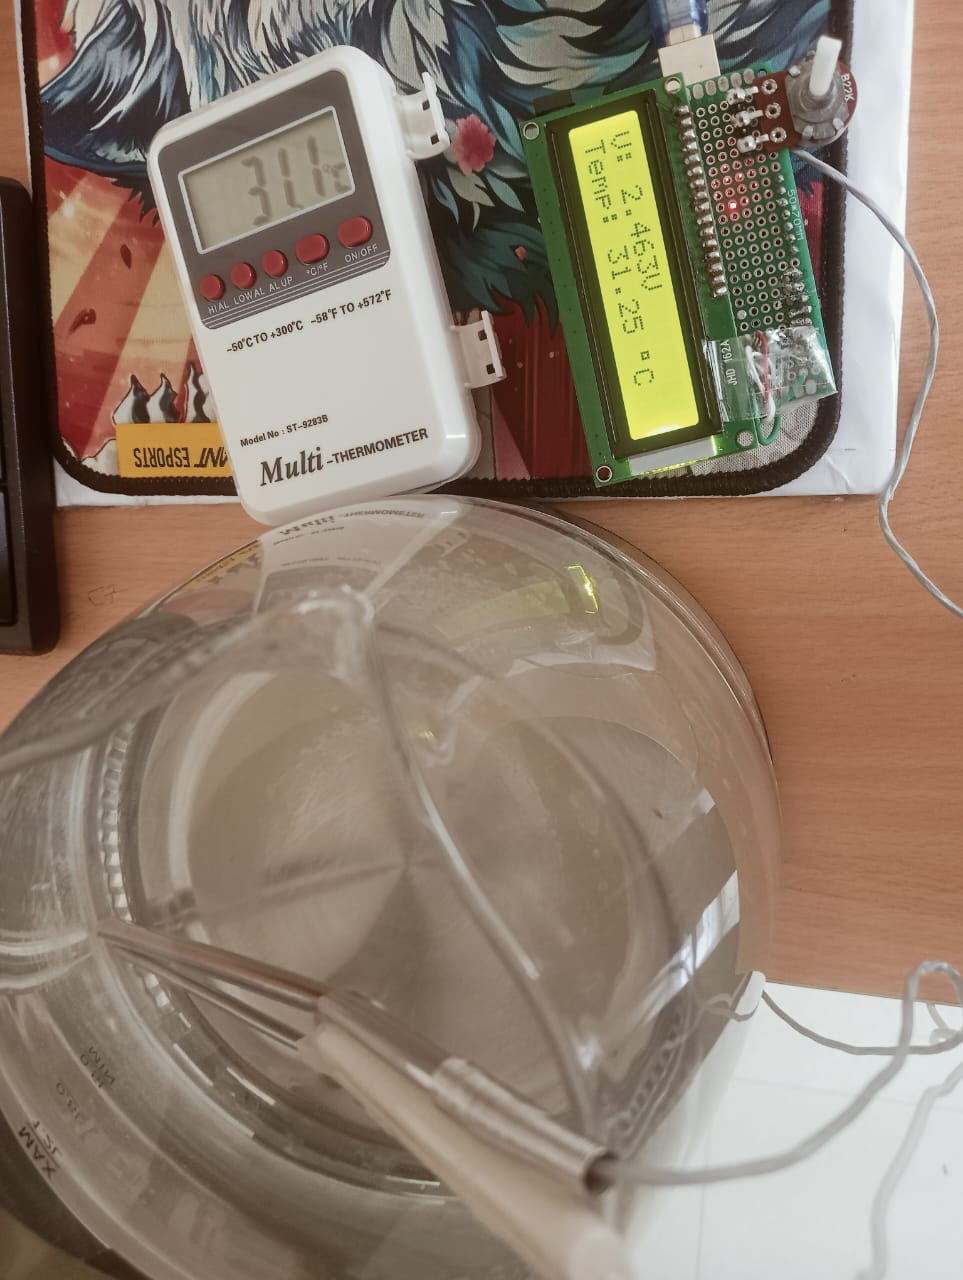
\includegraphics[width=0.75\columnwidth]{figs/demo1.jpeg}
    \caption{Project demonstration 1 alongside laboratory-grade thermometer.}
    \label{fig:demo1}
\end{figure}

\begin{figure}[H]
    \centering
    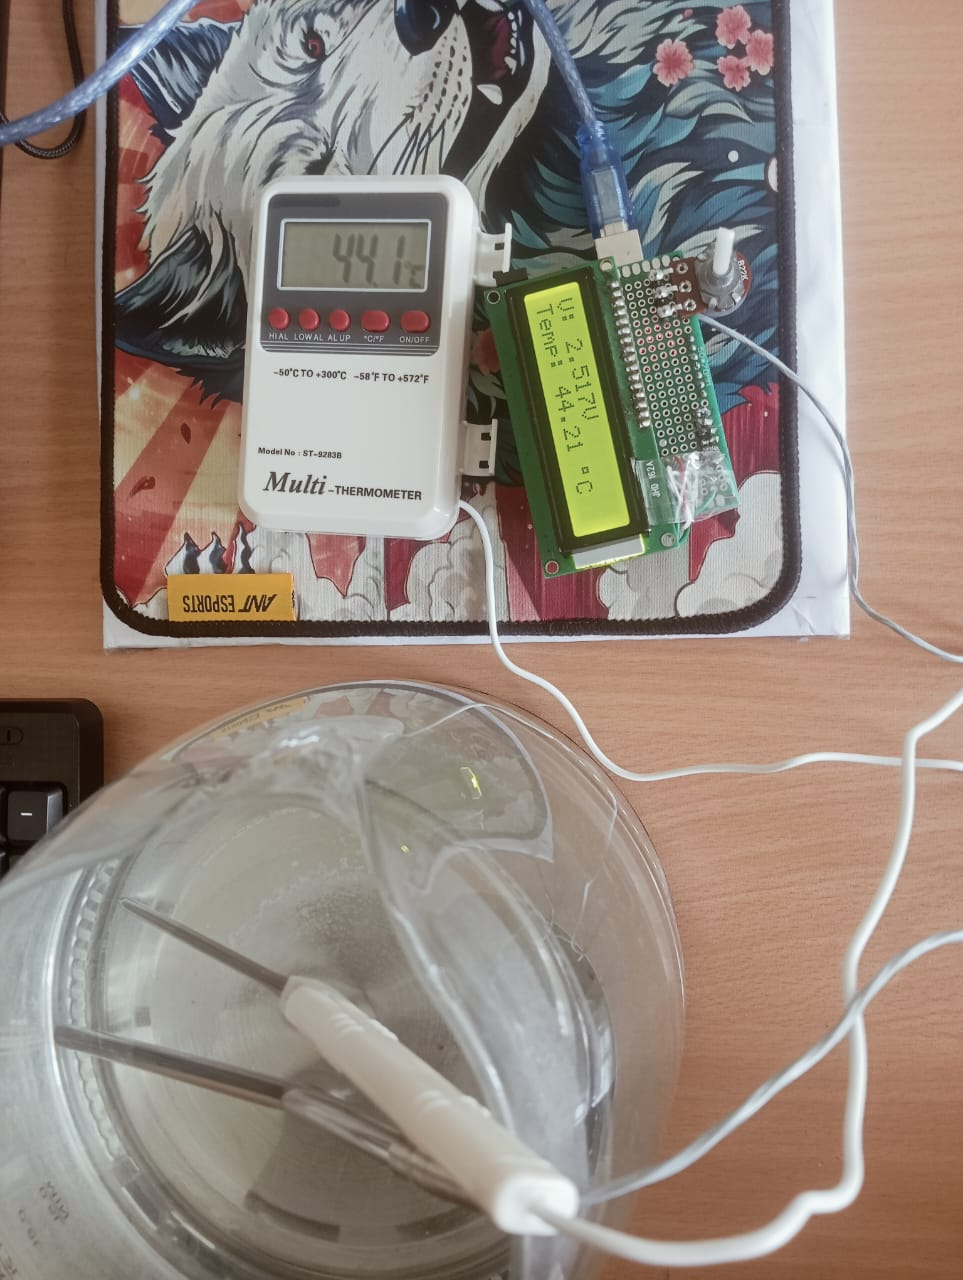
\includegraphics[width=0.75\columnwidth]{figs/demo2.jpeg}
    \caption{Project demonstration 2 alongside laboratory-grade thermometer.}
    \label{fig:demo2}
\end{figure}

\begin{figure}[H]
    \centering
    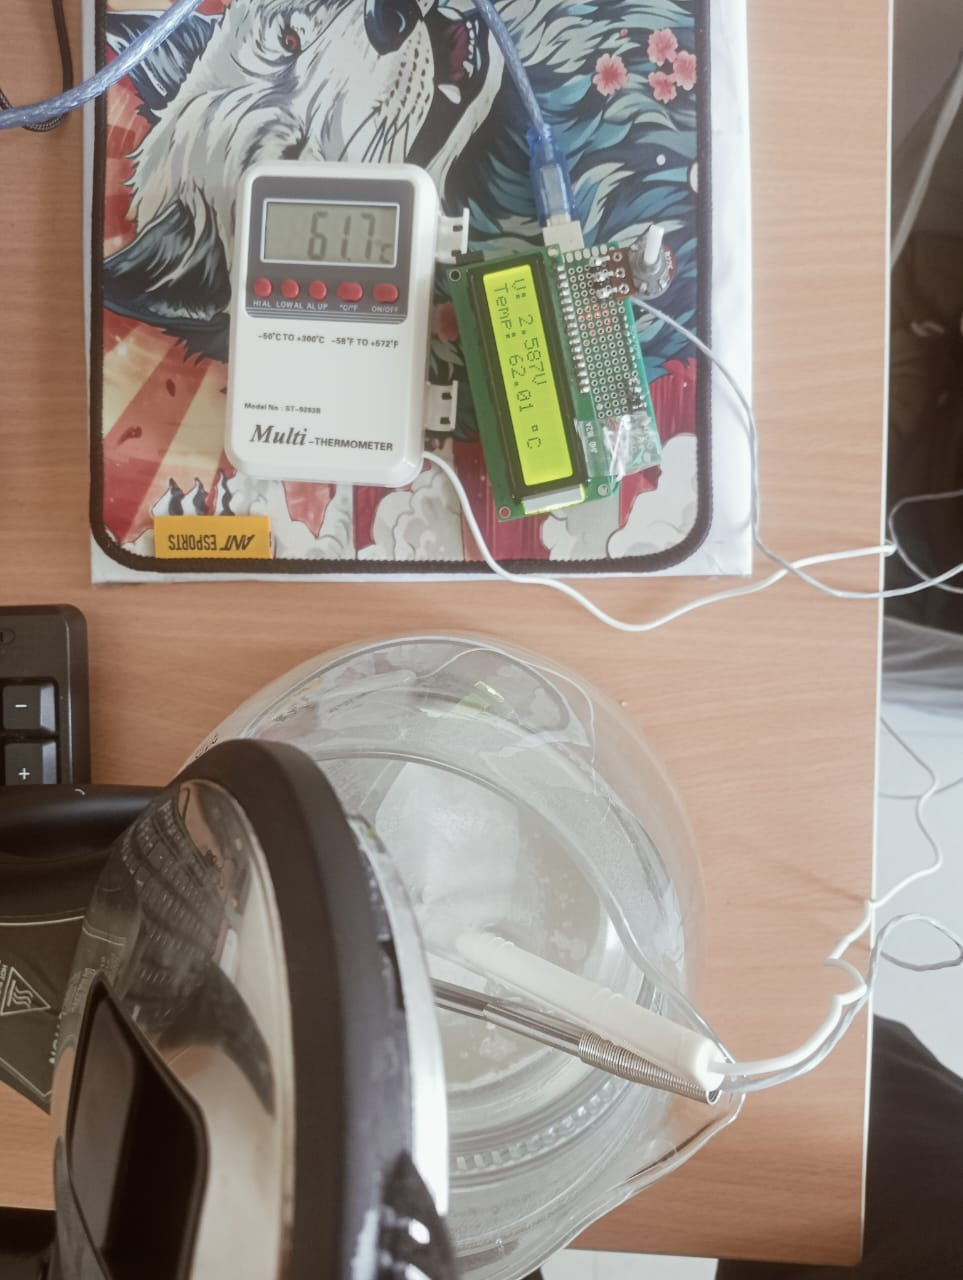
\includegraphics[width=0.75\columnwidth]{figs/demo3.jpeg}
    \caption{Project demonstration 3 alongside laboratory-grade thermometer.}
    \label{fig:demo3}
\end{figure}

\begin{figure}[H]
    \centering
    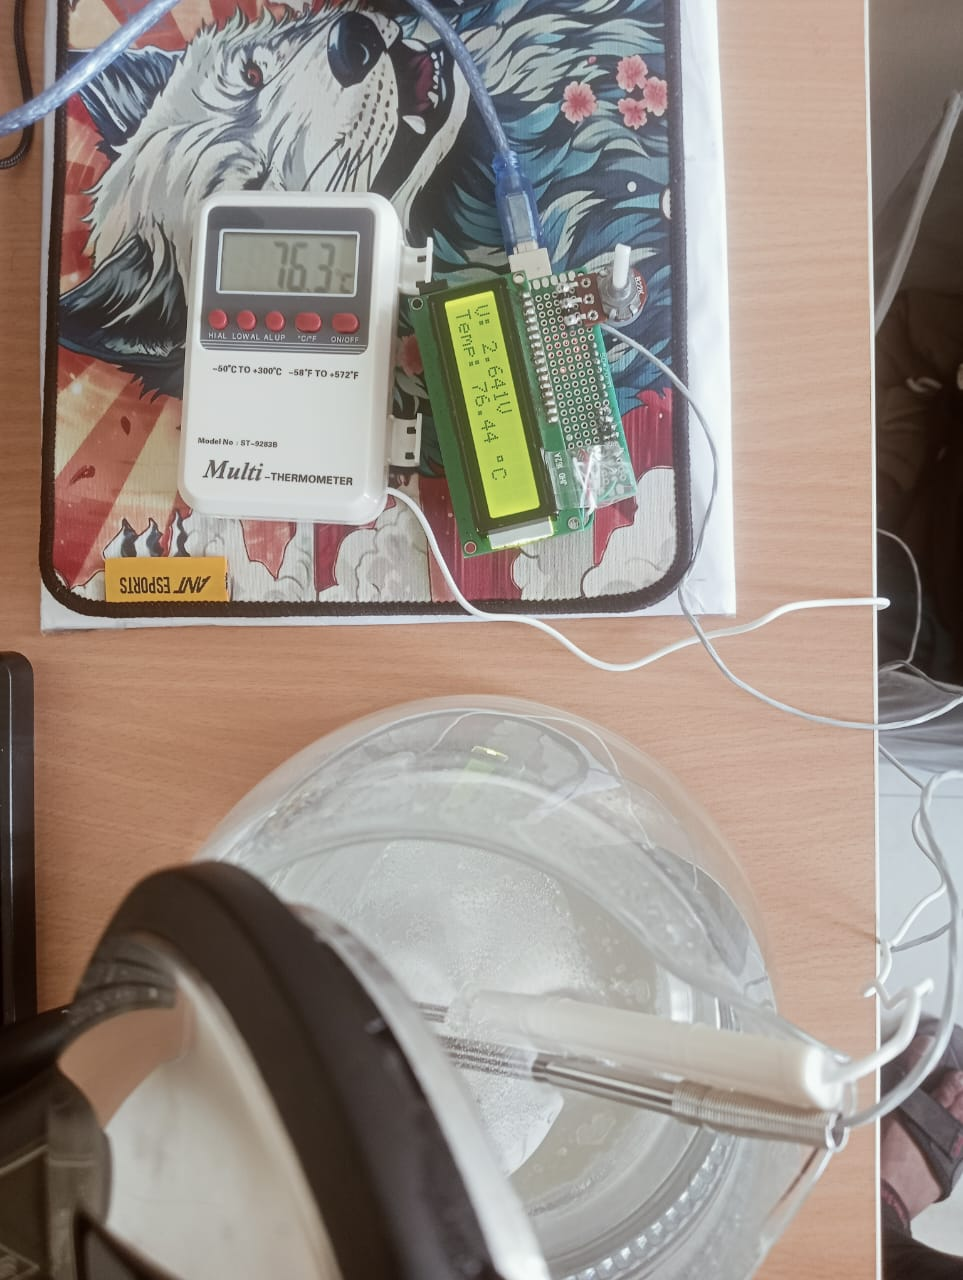
\includegraphics[width=0.75\columnwidth]{figs/demo4.jpeg}
    \caption{Project demonstration 4 alongside laboratory-grade thermometer.}
    \label{fig:demo4}
\end{figure}

\section{Key Takeaways}

This project helped us connect the theory of temperature-dependent
resistance to a working electronic measurement system. We learned that
temperature is not read directly by the Arduino: the sensor changes
resistance, the circuit turns that change into a voltage, the ADC
measures the voltage, and the code converts the measurement into a
temperature estimate. Following this chain made the relationship between
the physical sensor and the displayed value much more intuitive.

The project also taught us that debugging is a systematic process.
Faulty jumper wires initially made us suspect the LCD or Arduino, reversed
LCD data connections produced corrupted characters, and a solder bridge
made the PT100 path appear to have zero resistance. In each case, careful
inspection and multimeter measurements were more effective than changing
multiple parts at once.

Most importantly, we learned that a reliable instrument is built through
verification and calibration, not appearance alone. A polished enclosure
and additional features cannot compensate for an inaccurate measurement.
For a thermometer intended for industrial use, we would rather complete
tedious, repeatable calibration and minimise the measurement error than
make half-hearted innovations in secondary aspects of the design. The
priority is a dependable reading whose limitations are understood and
whose performance has been checked against a reference.

\ProjectImage{figs/finalcomplete_circuit.jpeg}
{Completed thermometer assembly, representing the outcome of the circuit-development process.}


\paragraph{Project demonstration}
The complete demo of this project can be found at
{\color[RGB]{0, 51, 153}\url{https://youtube.com/shorts/N8T5c-BsDCI?feature=share}}.

\end{document}
